
% \documentclass[border=10pt]{standalone}
% \usepackage{tikz}
% \usepackage{stmaryrd}

% \begin{document}
\begin{center}
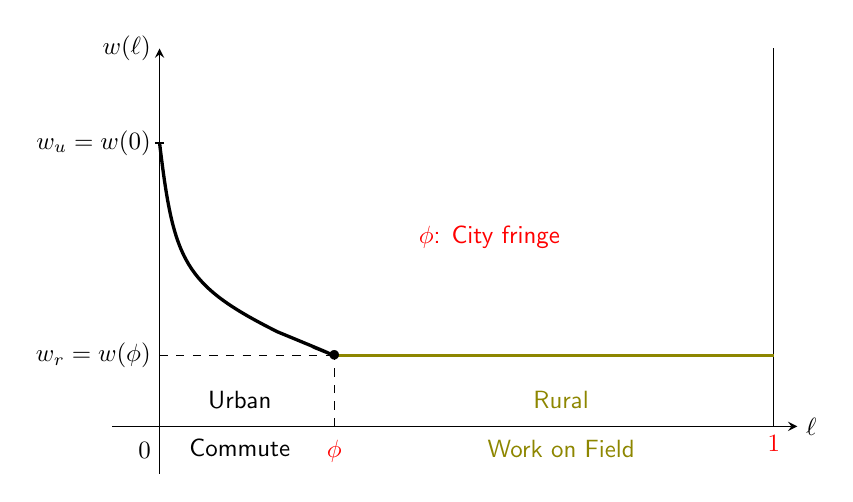
\begin{tikzpicture}[scale=0.6,every node/.style={scale=0.9}]

% xaxis
\draw[->,>=stealth,line width=0.5pt] (0,-1)--(0,8);
\draw (13.5,0) node (xaxis) [right] {$\ell$};
\draw[line width=0.5pt] (13,0)--(13,8);  % right y-axis
\draw (13,0) node [below] {\color{red}{$1$}};  % right y-axis label
\draw (0,-0.5) node (xaxis) [left] {$0$};
\draw[->,>=stealth,line width=0.5pt] (-1,0)--(13.5,0);%y axis


% axis labels

\uncover<2->{

\draw (0,8) node[left] {$w(\ell)$};  % yaxis label
% intercept of w(0)
\draw[line width=0.5pt] (-0.1,6)--(0.1,6);
\draw (0,6) node (yaxis) [left] {$w_u=w(0)$};}

\uncover<3->{
	% wage function
	\draw[line width=1.2pt, black] (0,6) ..controls +(0.3,-2.5) and +(-2,1).. (2.5,2) ..controls +(1.7,-0.7) and +(-0.5,0.2).. (3.7,1.5);
}


\uncover<4->{
% wage from phi to 1
\draw[line width=1.3pt,olive](3.7,1.5)--(13,1.5);

% dashed line for q(phi) and phi
\draw [dashed] (3.7,0) |-(3.7,1.5);
\draw [dashed] (0,1.5)--(3.7,1.5);
\draw (0,1.5) node [left] {$w_r=w(\phi)$};
\draw (3.7,1.5) node[black]{$\bullet$};
\draw (5.3,4) node[right] {\color{red}{$\phi$}\textsf{: City fringe}};
\draw (3.7,-0.1) node[below] {\color{red}{$\phi$}};

% text annotations
\draw (1.7,0.2) node[above] {\textsf{Urban}};
\draw (1.7,-0.08) node[below] {\textsf{Commute}};
\draw (8.5,0.2) node[above] {\textsf{\color{olive}{Rural}}};
\draw (8.5,-0.1) node[below] {\textsf{\color{olive}{Work on Field}}};}
\end{tikzpicture}
\end{center}

% \end{document}